\documentclass[11pt]{article}

% ---- encoding & fonts ----
\usepackage[utf8]{inputenc}
\usepackage[T1]{fontenc}
\usepackage{lmodern}
\usepackage{microtype}

% ---- math ----
\usepackage{amsmath,amssymb,amsthm,mathtools}

% ---- layout ----
\usepackage[margin=1in]{geometry}
\usepackage{enumitem}
\usepackage{booktabs}
\usepackage{array}
\usepackage{multirow}
\usepackage{caption}
\usepackage{xcolor}

% ---- graphics ----
\usepackage{tikz}
\usetikzlibrary{arrows.meta,positioning,fit,backgrounds,calc,shapes.geometric,quotes}

% ---- refs ----
\usepackage[round]{natbib}
\usepackage{hyperref}
\hypersetup{colorlinks=true, linkcolor=blue!50!black, citecolor=blue!50!black,
            urlcolor=blue!50!black}

% ---- theorem-like environments ----
\theoremstyle{definition}
\newtheorem{principle}{Principle}
\newtheorem{definition}{Definition}
\newtheorem{criterion}{Criterion}
\newtheorem{example}{Example}

\theoremstyle{remark}
\newtheorem{remark}{Remark}

% ---- macros ----
\newcommand{\state}[1]{\texttt{[#1]}}
\newcommand{\rel}[1]{\texttt{#1}}
\newcommand{\ntype}[1]{\textsc{#1}}
\newcommand{\ftpr}{\textsc{ftpr}}
\newcommand{\pfbench}{ParadigmForgeBench}
\newcommand{\PF}{ParadigmForge}

\title{\textbf{ParadigmForge}\\[2pt]
\large A Governed Architecture for Machine-Generated\\ Mathematical Theory Formation}

\author{Maximiliano Lucius\\
\small Independent Researcher / Aureus Technologies\\
\small \texttt{maximiliano@aureus-finance.com}}

\date{Draft --- July 2026}

\begin{document}
\maketitle

\begin{abstract}
\noindent
Autonomous and semi-autonomous systems increasingly produce plausible research-level
mathematics, and a growing body of work governs when a \emph{generated statement} may become
trusted knowledge. Proving statements inside a fixed formal language, however, is not the whole of
mathematical progress. Frontier mathematics has repeatedly advanced by \emph{changing the
representational and conceptual space} in which problems are posed---by inventing techniques,
building bridges between domains, and introducing new definitions, invariants, and objects that
expose previously hidden structure. We present \PF{}, a \emph{governed theory-formation
architecture} that extends the Bourbaki Engine research program from claim promotion to the
generation, testing, refinement, governance, and validation of candidate mathematical techniques,
cross-domain bridges, conceptual languages, and candidate domains. \PF{} organises discovery into
four escalating levels of novelty (novel technique; cross-domain bridge; new conceptual language;
domain genesis) and enforces a single governing principle: \emph{high epistemic temperature for
exploration, near-zero temperature for promotion}. A high-temperature speculative zone---Frontier
Atlas, TechniqueForge, BridgeForge, ConceptForge, Experimentarium, and DomainFoundry---proposes
radical candidates but holds \emph{no} authority to promote them; a near-zero-temperature trust
zone (the Mirador representation, formalization, and CongressBench adversarial review) alone may
admit a result into trusted knowledge, and every rejected proposal is retained as structured
negative knowledge. We contribute (i) an operational taxonomy of mathematical novelty; (ii) a
typed epistemic representation for techniques, bridges, concepts, failures, and candidate domains,
specified as an extension of Mirador; (iii) a discovery-to-promotion workflow that separates
speculative exploration from trusted knowledge; (iv) a multidimensional novelty model with explicit
anti-gaming controls that does not reduce novelty to textual or embedding distance; and (v)
\pfbench{}, a four-track evaluation framework for technique-, bridge-, concept-, and domain-level
novelty. We are explicit about maturity: \PF{} is an architecture and evaluation-framework
proposal built on the separately published Mirador and ProofContext prototypes; \textbf{no \PF{}
experiment has been run and no empirical result is claimed}. Every results table is a labelled
placeholder, and the complete execution plan is preregistered separately. The paper's argument is
deliberately conservative: mathematical AI will not reach frontier discovery merely by proving more
statements inside fixed languages; it must also learn to propose, test, reject, and govern changes
to the conceptual language of mathematics itself.
\end{abstract}

\tableofcontents

% =====================================================================
\section{Introduction}
\label{sec:intro}

A model that emits an unfamiliar-looking theorem has not, by that act, made a discovery. Whether a
statement constitutes progress depends on properties that fluency does not establish: it must be
true (or its falsity must be a useful counterexample), it must be novel, nontrivial, and useful to
subsequent work, and---at the frontier---it often must be expressible at all, which is not
guaranteed by the language currently available. The last point is the concern of this paper.
Much recent progress in AI for mathematics has been organised around a fixed target language: given
a statement in Lean or in natural language, produce a derivation a checker accepts
\citep{polu2020,yang2023leandojo,trinh2024alphageom}. This is the right frame for olympiad-style
problems and for filling a known gap in a formal library, and it has produced striking results.
But research mathematics is not only the discharge of statements in a fixed language. Its most
consequential moves are frequently changes to the language itself: a new technique that makes a
previously intractable estimate routine; a bridge that transports a theorem from one domain to
another; a definition or invariant that compresses several disconnected phenomena into one; and,
occasionally, the emergence of an entire productive domain around such a language.

The Bourbaki Engine program \citep{lucius2026bourbaki} has developed an infrastructure for the
\emph{governance} of machine-assisted mathematics: a typed, versioned representation whose unit is
a Mathematical Cell \citep{lucius2026mirador}; a dependency-aware retriever that returns the
minimal verifiable context in which a claim can be used safely \citep{lucius2026proofcontext}; a
propose-only discovery plane of operators \citep{lucius2026theoryforge}; a benchmark for the
reliability of adversarial review \citep{lucius2026congressbench}; and a benchmark for faithful
ingestion of the literature \citep{lucius2026mathingest}. The spine of that program is the
separation of a Discovery Plane, which may be speculative and internally contradictory, from a
Trust Plane, which alone may promote a claim into load-bearing knowledge. That program governs
\emph{accumulation}. It does not, on its own, address the production of new representational and
conceptual structure. A machine that only prevents false promotions can sit forever at an empty
frontier.

\paragraph{Contribution of this paper.}
\PF{} extends the Bourbaki Engine from governed claim promotion to \emph{governed theory
formation}. It is a layer above TheoryForge that targets the creation, testing, and adversarial
validation of \emph{techniques}, \emph{cross-domain bridges}, \emph{conceptual languages}, and
\emph{candidate domains}---not merely conjectures and reductions inside an existing theory. Its
central design commitment is a governed separation of temperatures: a high-temperature speculative
zone proposes radical candidates without any promotion authority, and a near-zero-temperature trust
zone admits results only through formalization and fresh-context adversarial review, retaining
every rejection as structured negative knowledge (Fig.~\ref{fig:arch}).

\paragraph{Maturity, stated plainly.}
This is an \emph{architecture and evaluation-framework} paper. The substrates it depends on
(Mirador, ProofContext) are separately published prototypes; the \PF{} layer itself is specified,
not built. \textbf{No \PF{} experiment has been run, and this paper reports no accuracy, success
rate, expert assessment, or mathematical discovery.} Results tables appear only as clearly marked
placeholders; the executable experimental program is preregistered in the accompanying roadmap. We
adopt the companion program's evidential discipline throughout: components are labelled
\emph{implemented}, \emph{specified}, or \emph{planned}, and design goals are never written as if
measured.

\paragraph{Research questions.}
The paper is organised around six questions, none of which it answers empirically; it specifies how
each becomes answerable.
\begin{description}[leftmargin=2.4em,style=nextline,itemsep=1pt]
  \item[RQ1] Can a governed AI system reconstruct mathematically productive \emph{techniques} from
  pre-discovery knowledge, without collapsing into memorised rediscovery?
  \item[RQ2] Can typed structural alignment produce \emph{theorem-transporting} bridges that
  outperform semantic analogy?
  \item[RQ3] Can an AI-generated \emph{concept} demonstrate explanatory compression and predictive
  utility on held-out mathematical cases?
  \item[RQ4] Which governance mechanisms most effectively prevent cosmetic novelty and false theory
  promotion?
  \item[RQ5] What evidence is sufficient to distinguish a \emph{productive mathematical domain} from
  an overfitted collection of definitions?
  \item[RQ6] Does structured \emph{negative knowledge} improve mathematical exploration by
  preventing repeated failure?
\end{description}

\paragraph{Claims.}
We claim, as architectural and methodological contributions only:
(1) a governed architecture for machine-assisted mathematical theory formation
(\S\ref{sec:arch});
(2) an operational taxonomy of mathematical novelty (\S\ref{sec:arch}, \S\ref{sec:novelty});
(3) a typed representation for techniques, bridges, concepts, failures, and candidate domains
(\S\ref{sec:repr});
(4) a discovery-to-promotion workflow separating speculative exploration from trusted knowledge
(\S\ref{sec:principles}, \S\ref{sec:governance});
(5) \pfbench{}, an evaluation framework for technique-, bridge-, concept-, and domain-level novelty
(\S\ref{sec:bench});
(6) a research methodology for testing mathematical productivity without conflating it with textual
novelty (\S\ref{sec:method}); and
(7) an extension of the Bourbaki Engine toward controlled conceptual evolution (\S\ref{sec:bourbaki}).
No claim in this paper depends on an experiment we have not run.

\begin{figure}[t]
\centering
\resizebox{\textwidth}{!}{% Full ParadigmForge architecture: speculative zone, membrane, trust zone.
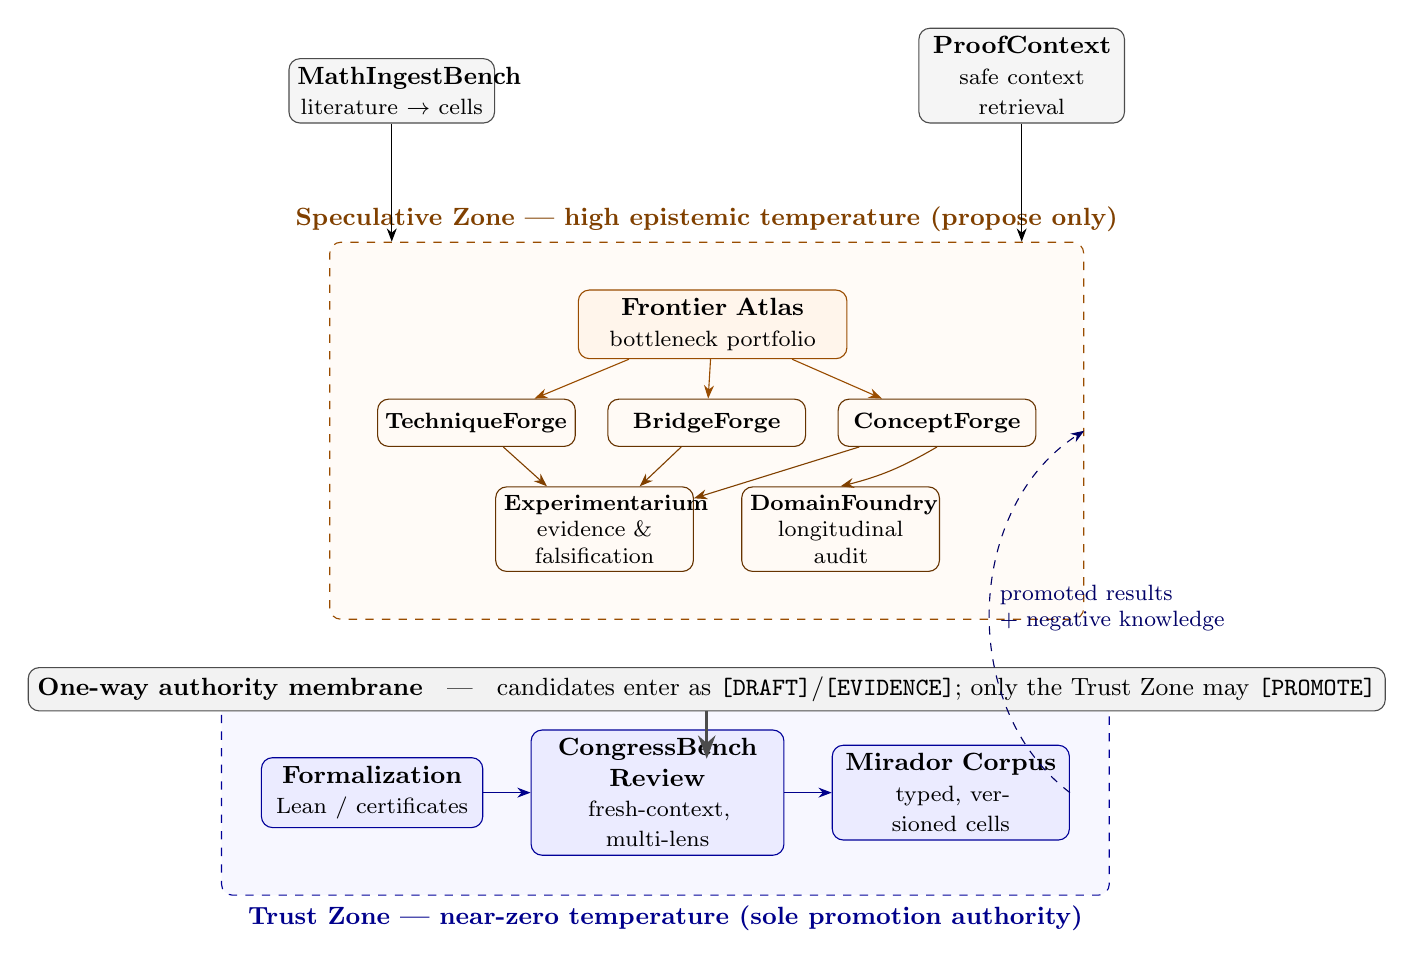
\begin{tikzpicture}[
    font=\small,
    box/.style={draw, rounded corners, align=center, minimum height=7mm,
                inner sep=3pt, text width=26mm},
    spec/.style={box, fill=orange!8, draw=orange!60!black},
    trust/.style={box, fill=blue!8, draw=blue!60!black},
    sub/.style={box, fill=orange!4, draw=orange!40!black, text width=23mm,
                minimum height=6mm, font=\footnotesize},
    io/.style={box, fill=gray!8, draw=gray!60!black, text width=24mm},
    >=Stealth,
    ]

% ---- Discovery / speculative zone ----
\node[spec, text width=32mm] (atlas) {\textbf{Frontier Atlas}\\\footnotesize bottleneck portfolio};
\node[sub, below=5mm of atlas, xshift=-30mm] (tech) {\textbf{TechniqueForge}};
\node[sub, right=4mm of tech] (bridge) {\textbf{BridgeForge}};
\node[sub, right=4mm of bridge] (concept) {\textbf{ConceptForge}};
\node[sub, below=5mm of tech, xshift=15mm] (exp) {\textbf{Experimentarium}\\\footnotesize evidence \& falsification};
\node[sub, right=6mm of exp] (foundry) {\textbf{DomainFoundry}\\\footnotesize longitudinal audit};

\begin{scope}[on background layer]
  \node[draw=orange!60!black, dashed, rounded corners, fill=orange!3,
        fit=(atlas)(tech)(concept)(exp)(foundry),
        inner sep=6mm, label={[orange!50!black]above:\textbf{Speculative Zone --- high epistemic temperature (propose only)}}] (speczone) {};
\end{scope}

% ---- Trust zone ----
\node[trust, below=20mm of exp, xshift=8mm, text width=30mm] (congress) {\textbf{CongressBench Review}\\\footnotesize fresh-context, multi-lens};
\node[trust, left=6mm of congress, text width=26mm] (formal) {\textbf{Formalization}\\\footnotesize Lean / certificates};
\node[trust, right=6mm of congress, text width=28mm] (mirador) {\textbf{Mirador Corpus}\\\footnotesize typed, versioned cells};

\begin{scope}[on background layer]
  \node[draw=blue!60!black, dashed, rounded corners, fill=blue!3,
        fit=(formal)(congress)(mirador),
        inner sep=5mm, label={[blue!55!black]below:\textbf{Trust Zone --- near-zero temperature (sole promotion authority)}}] (trustzone) {};
\end{scope}

% ---- Membrane ----
\node[draw=black!70, fill=black!5, rounded corners, minimum width=120mm,
      minimum height=5mm, below=6mm of speczone.south, anchor=north,
      align=center] (membrane)
      {\textbf{One-way authority membrane} \; --- \; candidates enter as \texttt{[DRAFT]}/\texttt{[EVIDENCE]}; only the Trust Zone may \texttt{[PROMOTE]}};

% ---- external I/O ----
\node[io, above=15mm of speczone.north, xshift=-40mm] (ingest) {\textbf{MathIngestBench}\\\footnotesize literature $\to$ cells};
\node[io, above=15mm of speczone.north, xshift=40mm] (retr) {\textbf{ProofContext}\\\footnotesize safe context retrieval};

% ---- edges ----
\draw[->] (ingest) -- (speczone.north -| ingest);
\draw[->] (retr) -- (speczone.north -| retr);
\draw[->, orange!60!black] (atlas) -- (tech);
\draw[->, orange!60!black] (atlas) -- (bridge);
\draw[->, orange!60!black] (atlas) -- (concept);
\draw[->, orange!50!black] (tech) -- (exp);
\draw[->, orange!50!black] (concept) -- (exp);
\draw[->, orange!50!black] (bridge) -- (exp);
\draw[->, orange!50!black] (concept.south) to[bend left=8] (foundry.north);

\draw[->, very thick, black!70] (membrane.south) -- ++(0,-6mm);
\draw[->, blue!55!black] (formal) -- (congress);
\draw[->, blue!55!black] (congress) -- (mirador);
% feedback loop: promoted knowledge and negative knowledge back to Atlas
\draw[->, blue!40!black, dashed] (mirador.east) to[bend left=55]
      node[pos=0.5,right,align=left,font=\footnotesize]{promoted results\\+ negative knowledge}
      (speczone.east);
\end{tikzpicture}
}
\caption{The \PF{} architecture. A high-temperature \emph{speculative zone} (orange) proposes
candidates but holds no promotion authority; a near-zero-temperature \emph{trust zone} (blue) alone
admits results into the Mirador corpus, through formalization and CongressBench review. The two are
joined by a one-way authority membrane. MathIngestBench feeds the corpus the Frontier Atlas reads;
ProofContext supplies safe context; promoted results \emph{and} negative knowledge flow back to the
Atlas. Every component has an evaluation mechanism (\S\ref{sec:bench}).}
\label{fig:arch}
\end{figure}

% =====================================================================
\section{From Theorem Proving to Theory Formation}
\label{sec:proving-to-forming}

We fix a set of distinctions that the rest of the paper depends on. Each names a boundary that is
easy to blur and expensive to blur.

\begin{description}[leftmargin=1.4em,itemsep=2pt]
  \item[Theorem proving vs.\ theory formation.] Proving derives a fixed statement inside a fixed
  language. Theory formation changes what statements are available to prove: it introduces
  definitions, invariants, techniques, and translations, and only then proves within the enlarged
  language. The former has a well-posed success predicate (a checker accepts); the latter does not,
  which is precisely why it needs governance rather than a single score.
  \item[Conjecture generation vs.\ conceptual invention.] A conjecture is a statement in the
  existing language whose truth is open. A concept is a new piece of language---an object, an
  equivalence, an invariant---whose value is not truth but productivity. A system can generate
  endless conjectures without inventing a single concept.
  \item[Analogy vs.\ a valid mathematical bridge.] An analogy asserts resemblance. A bridge is a
  typed, partial, structure-preserving map that \emph{transports} at least one nontrivial theorem
  and states where it breaks. Analogy is cheap; transport is the evidence.
  \item[Renaming vs.\ genuine abstraction.] Renaming preserves content-hash identity
  \citep{lucius2026mirador}; abstraction changes which theorems are provable or which proofs are
  shorter. The first is detectable mechanically; the second must be demonstrated.
  \item[Local novelty vs.\ productive novelty.] A construction can be new-to-the-corpus yet inert.
  Productive novelty yields theorems, transfers across problems, and is used by agents other than
  its proposer.
  \item[Empirical evidence vs.\ proof.] Exact enumeration, simulation, and pattern-finding generate
  evidence and falsification pressure; they do not establish theorems. A numeric grid is never a
  proof \citep{lucius2026bourbaki}.
  \item[Discovery vs.\ epistemic promotion.] Producing a candidate is discovery in the weak sense;
  admitting it as trusted knowledge is promotion, a governed act with a different authority.
  \item[Open-ended exploration vs.\ trusted knowledge.] The two require opposite virtues---diversity
  and permissiveness on one side, conservatism and auditability on the other---and must not share
  authority.
\end{description}

\noindent
These distinctions are not rhetorical. Each corresponds to a concrete failure mode that \PF{} is
built to detect: renaming as novelty, analogy without transport, evidence promoted as proof, a
concept fitted only to the examples that motivated it. \S\ref{sec:novelty} makes each measurable.

The literature of \emph{automated theory formation} is older than the current wave of language
models. Lenat's \textsc{am} explored concepts and conjectures by heuristic search
\citep{lenat1976am}; Colton's \textsc{hr} systematised concept invention and the problem of
``interestingness'' \citep{colton2002hr}. Lakatos gave the philosophical account that this paper
operationalises: mathematical knowledge grows not by monotone accumulation but by the interplay of
conjecture, proof, and refutation, in which counterexamples reshape definitions themselves
\citep{lakatos1976}. \PF{} can be read as a governed, machine-scale realisation of that dialectic,
with the crucial addition---absent from the classical systems---of an explicit separation between
proposing and promoting.

% =====================================================================
\section{Background and Related Work}
\label{sec:related}

We situate \PF{} against seven strands of work, citing primary sources and marking, for each,
the boundary \PF{} adds. We claim novelty only in the composition, not in any single mechanism.

\paragraph{Automated and formal theorem proving.}
The mechanisation of proof runs from the Logic Theory Machine \citep{newell1957} and proof planning
\citep{bundy1988} to McCune's resolution of the Robbins conjecture \citep{mccune1997}, and to the
large computer-assisted and formal proofs that fixed the modern standard of certified computation:
the Four Colour Theorem \citep{gonthier2008}, the Kepler conjecture \citep{hales2017}, and the
Boolean Pythagorean triples problem \citep{heule2016}. Interactive proof assistants---Lean 4 and
its library \citep{demoura2021lean4,mathlib2020}---supply the trusted kernels \PF{} treats as one
verification backend among several. This lineage certifies proofs; it does not generate techniques
or concepts.

\paragraph{Neural and LLM theorem proving.}
Learned provers---GPT-$f$ \citep{polu2020}, HyperTree Proof Search \citep{lample2022htps},
retrieval-augmented proving with LeanDojo \citep{yang2023leandojo}, and the DeepSeek-Prover line
\citep{xin2024dsprover,xin2024dsproverv15}---search for derivations of \emph{given} statements, and
autoformalization aligns informal statements to formal ones \citep{wu2022autoform,jiang2023dsp}.
Benchmarks such as miniF2F \citep{zheng2022minif2f}, the MATH dataset \citep{hendrycks2021math},
GSM8K \citep{cobbe2021gsm8k}, Minerva \citep{lewkowycz2022minerva}, and FrontierMath
\citep{glazer2024frontiermath} measure proving or problem-solving on fixed statements, and
research-level benchmarks such as First Proof \citep{abouzaid2026firstproof} raise the difficulty to
unpublished problems---but all still score derivation of a \emph{given} statement. \PF{} consumes
such provers as components but is evaluated on a different axis: the productivity of newly proposed
language.

\paragraph{AI-assisted discovery.}
AlphaGeometry and its successor solve olympiad geometry by coupling a language model to a symbolic
engine with auxiliary-construction search \citep{trinh2024alphageom,chervonyi2025alphageom2};
AlphaProof reached competition-level formal proving \citep{deepmind2024alphaproof}. Program-search
discovery---FunSearch \citep{romera2024funsearch} and AlphaEvolve
\citep{deepmind2025alphaevolve}---optimises an executable against a fixed evaluator and has produced
genuinely new constructions (e.g.\ improved cap-set and packing bounds). These systems change
\emph{artifacts} against a fixed objective; \PF{} targets change to the \emph{objective language}
itself, under governance, and measures it by transfer and productivity rather than by a single
evaluator score. Davies et al.\ showed AI can guide human mathematical intuition toward new theorems
\citep{davies2021}; \PF{} aims to make the intuition-shaping step itself an auditable, governed
artifact.

\paragraph{Open-ended search and quality--diversity.}
The exploration side of \PF{} inherits from novelty search \citep{lehman2011novelty} and
quality--diversity methods such as MAP-Elites \citep{mouret2015mapelites,cully2015}, which maintain
diverse populations rather than optimising a scalar. \PF{}'s speculative zone is a quality--diversity
population over \emph{typed mathematical objects}, with the essential addition that diversity is not
enough: a candidate must survive transport, falsification, and adversarial review before it counts.

\paragraph{Analogy and structural transfer.}
Structure-mapping theory formalises analogy as alignment of relational structure rather than surface
features \citep{gentner1983}. BridgeForge (\S\ref{sec:bridgeforge}) is a mathematical,
transport-obligated realisation of that idea: alignment is necessary but insufficient; the bridge
must carry a theorem and declare its breakage point.

\paragraph{Mathematical knowledge representation, provenance, and truth maintenance.}
Truth-maintenance systems introduced epistemic states and dependency-directed invalidation
\citep{doyle1979tms,dekleer1986atms}; provenance and transparent-log methods
\citep{kuhn2016nanopub,moreau2013prov,laurie2013ct} and build-level invalidation \citep{celik2017icoq}
inform the Mirador substrate. \PF{} extends that substrate with node and relation types for
theory formation (\S\ref{sec:repr}).

\paragraph{Philosophy and practice of mathematical discovery.}
Beyond Lakatos \citep{lakatos1976} and P\'olya \citep{polya1945}, the paper takes seriously the
measure-of-intelligence view that genuine novelty is skill-acquisition on unseen structure, not
recall \citep{chollet2019}; this motivates the contamination controls and held-out designs of
\S\ref{sec:bench}.

\begin{table}[t]
\centering
\small
\caption{Capability comparison with representative systems. $\bullet$ = provided;
$\circ$ = partial or scoped; -- = not provided. Columns: \emph{Prove} a fixed statement;
generate \emph{Conj}ectures; synthesise \emph{Conc}epts / definitions; construct cross-domain
\emph{Bridge}s with theorem transport; \emph{Gov}erned promotion (separation of powers);
retain structured \emph{Neg}ative knowledge. Cells for \PF{} denote capabilities the architecture
\emph{specifies}; the layer is not yet implemented (\S\ref{sec:limits}).}
\label{tab:compare}
\resizebox{\textwidth}{!}{%
\begin{tabular}{lcccccc}
\toprule
System & Prove & Conj & Conc & Bridge & Gov & Neg \\
\midrule
Lean / mathlib \citep{demoura2021lean4,mathlib2020} & $\bullet$ & -- & -- & -- & $\circ$ & -- \\
AlphaGeometry(2) \citep{trinh2024alphageom,chervonyi2025alphageom2} & $\bullet$ & $\circ$ & -- & -- & -- & -- \\
DeepSeek-Prover \citep{xin2024dsproverv15} & $\bullet$ & -- & -- & -- & -- & -- \\
FunSearch / AlphaEvolve \citep{romera2024funsearch,deepmind2025alphaevolve} & $\circ$ & $\circ$ & -- & -- & $\circ$ & -- \\
TheoryForge \citep{lucius2026theoryforge} & $\circ$ & $\bullet$ & $\circ$ & $\circ$ & $\bullet$ & $\circ$ \\
\textbf{\PF{}} (this paper) & $\circ$ & $\bullet$ & $\bullet$ & $\bullet$ & $\bullet$ & $\bullet$ \\
\bottomrule
\end{tabular}}
\end{table}

% =====================================================================
\section{Bourbaki Engine Context}
\label{sec:bourbaki}

\PF{} is not an isolated system; it is an extension of an existing, partly implemented program.
We summarise the substrate so the paper is self-contained.

\begin{description}[leftmargin=1.4em,itemsep=2pt]
  \item[Mirador] \citep{lucius2026mirador} represents mathematical knowledge as a
  typed, versioned \emph{Mathematical Cell}: a canonical claim bound to its context (assumptions,
  exclusions, regularity, scope), typed dependency edges (each carrying its own soundness
  obligation), artifacts, provenance, and an \emph{epistemic state}. Two commitments are
  load-bearing for \PF{}: object \emph{type} is orthogonal to epistemic \emph{state} (being a
  ``theorem'' does not make a cell \state{PROMOTED}); and claim identity is the canonical hash of
  statement-plus-context, so a mere renaming collides with its source and cannot be sold as new.
  Invalidation propagates deterministically over an append-only, hash-chained event log.
  \item[ProofContext] \citep{lucius2026proofcontext} compiles a query into a typed Problem
  Signature and returns the smallest \emph{Evidence Bundle} in which a claim can be used safely,
  rejecting near-matches that are incompatible on a typed axis regardless of similarity, and holding
  no authority to promote.
  \item[TheoryForge] \citep{lucius2026theoryforge} is the propose-only Discovery Plane: a library of
  operators emitting typed candidate cells at epistemic state at most \state{EVIDENCE}.
  \item[CongressBench] \citep{lucius2026congressbench} measures the \emph{False Theorem Promotion
  Rate} (\ftpr{}) of adversarial, fresh-context review across a ladder of reviewer independence.
  \item[MathIngestBench] \citep{lucius2026mathingest} measures faithful ingestion of the literature
  into cells---the front of the pipeline that populates the corpus the Frontier Atlas reads.
  \item[Bourbaki Engine] \citep{lucius2026bourbaki} composes these into a two-plane architecture
  (Discovery vs.\ Trust) with a one-way authority membrane, certificate discipline
  ($\text{search} \neq \text{evidence} \neq \text{certificate} \neq \text{checker}$), and a
  readiness ladder $R0$--$R9$ whose top rungs the engine cannot self-declare.
\end{description}

\PF{} occupies a specific place in that ladder. The engine's ladder reaches, at $R3$--$R4$, the
regeneration of nontrivial known results and the production of a genuinely new lemma, counterexample,
reduction, or barrier on a bounded open problem. \PF{} is the machinery aimed at that transition and
beyond: where TheoryForge proposes conjectures and reductions \emph{inside} a language, \PF{}
proposes and governs changes \emph{to} the language---techniques, bridges, concepts, and, over long
horizons, domains. It reuses Mirador for representation, ProofContext for retrieval, and a
CongressBench-compatible reviewer for review; it adds the six components of \S\ref{sec:arch}, the
typed extensions of \S\ref{sec:repr}, and the evaluation framework of \S\ref{sec:bench}.

% =====================================================================
\section{Design Principles}
\label{sec:principles}

The architecture follows from a small number of principles. Each is stated so that a design that
violates it can be identified.

\begin{principle}[Representational change is a first-class goal]
\label{prin:repr}
The system's objective is not only to prove statements in a fixed language but to propose, test, and
govern changes to that language: new techniques, bridges, concepts, and---emergently---domains.
Success is measured by productivity and transfer, not only by proof accuracy.
\end{principle}

\begin{principle}[Temperature separation]
\label{prin:temp}
\emph{High epistemic temperature for exploration; near-zero epistemic temperature for promotion.}
Speculative agents may propose radical, imperfect, even internally contradictory ideas; they must
never promote their own results into trusted knowledge. Promotion is a distinct, conservative act
performed by an independent authority.
\end{principle}

\begin{principle}[Transport over resemblance]
\label{prin:transport}
A proposed bridge or analogy counts only if it transports a nontrivial mathematical statement and
states where it fails. Semantic similarity proposes; a checkable transport adjudicates.
\end{principle}

\begin{principle}[Necessity over decoration]
\label{prin:necessity}
A proposed technique or concept counts only if an ablation shows its new component is
\emph{counterfactually necessary}---that removing it fails to close the target obligation or loses
the theorem yield. Aesthetic reformulation without necessity is rejected.
\end{principle}

\begin{principle}[Productivity, not proclamation]
\label{prin:productivity}
A ``new domain'' cannot be declared by an agent. It is recognised only through sustained
productivity: a family of objects, internal operations and invariants, multiple theorems across
more than one problem family, natural internal questions, transfer to established domains, and use
by agents other than the proposer.
\end{principle}

\begin{principle}[Failure is knowledge]
\label{prin:failure}
Rejected proposals are not discarded. Each is retained as structured negative knowledge---a failed
approach, a counterexample, an obstruction or barrier certificate, with an explanation of \emph{why}
it fails---and reused to prune future exploration.
\end{principle}

\begin{principle}[Novelty is multidimensional]
\label{prin:novelty}
Mathematical novelty is not textual, embedding, or retrieval distance. It is a vector of structural
change, operational change, explanatory compression, theorem productivity, transfer breadth,
counterfactual necessity, robustness, independent rediscovery, and verification coverage. No scalar
fully determines it.
\end{principle}

Principles~\ref{prin:temp} and~\ref{prin:failure} are the governance core; \ref{prin:transport}
and~\ref{prin:necessity} are the anti-gaming core; \ref{prin:productivity} is the criterion that
keeps ``domain'' honest.

% =====================================================================
\section{ParadigmForge Architecture}
\label{sec:arch}

\PF{} comprises six components in the speculative zone and a governance path into the trust zone
(Fig.~\ref{fig:arch}). We specify each by its input, its output (always typed Mirador cells at
epistemic state at most \state{EVIDENCE}), its operators, and---critically---its \emph{acceptance
gate}, the check a candidate must survive to leave the component. Every component has a corresponding
evaluation mechanism in \S\ref{sec:bench}.

The four levels of novelty the architecture is designed to reach are shown in
Fig.~\ref{fig:levels}. They are escalating in representational change and in difficulty of
validation; a system may operate productively at $L1$ for a long time before any $L3$ candidate
survives.

\begin{figure}[t]
\centering
\resizebox{0.92\textwidth}{!}{% Four escalating levels of mathematical novelty as a staircase.
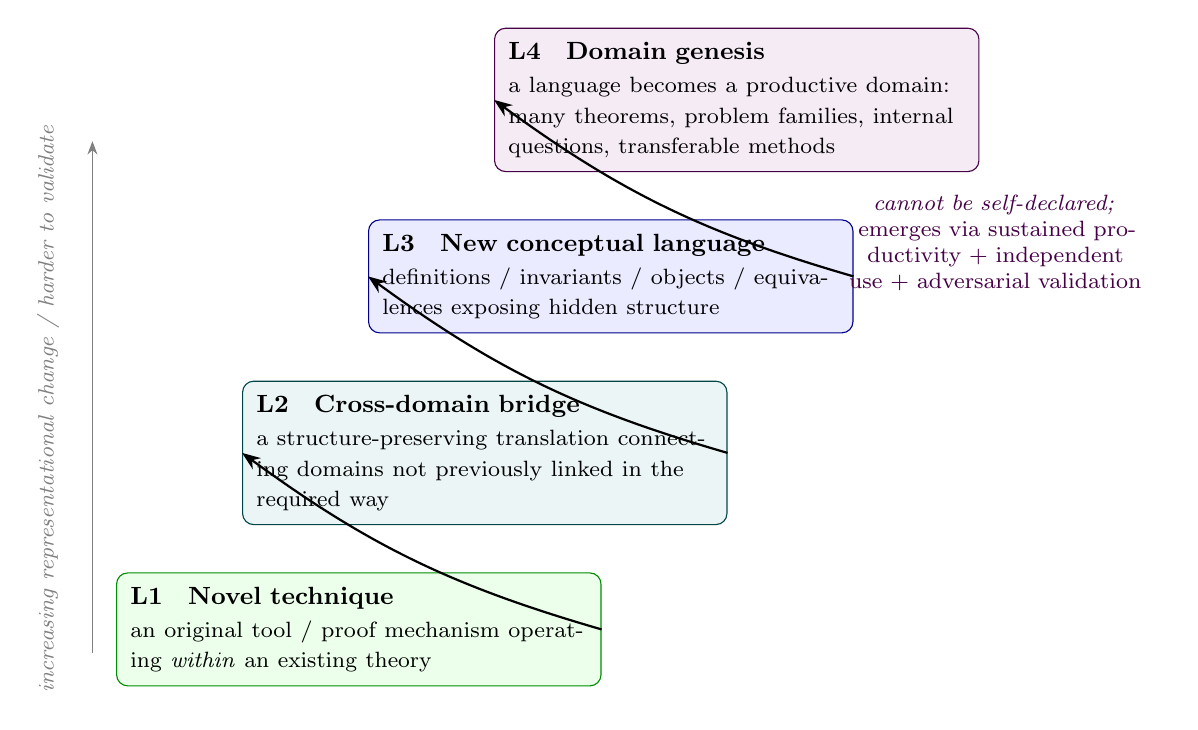
\begin{tikzpicture}[
    font=\small,
    lvl/.style={draw, rounded corners, align=left, inner sep=5pt,
                text width=58mm, minimum height=11mm},
    l1/.style={lvl, fill=green!8, draw=green!55!black},
    l2/.style={lvl, fill=teal!8, draw=teal!55!black},
    l3/.style={lvl, fill=blue!8, draw=blue!55!black},
    l4/.style={lvl, fill=violet!8, draw=violet!55!black},
    >=Stealth,
    ]
\node[l1] (l1) {\textbf{L1 \; Novel technique}\\[1pt]\footnotesize an original tool / proof mechanism operating \emph{within} an existing theory};
\node[l2, above=6mm of l1, xshift=16mm] (l2) {\textbf{L2 \; Cross-domain bridge}\\[1pt]\footnotesize a structure-preserving translation connecting domains not previously linked in the required way};
\node[l3, above=6mm of l2, xshift=16mm] (l3) {\textbf{L3 \; New conceptual language}\\[1pt]\footnotesize definitions / invariants / objects / equivalences exposing hidden structure};
\node[l4, above=6mm of l3, xshift=16mm] (l4) {\textbf{L4 \; Domain genesis}\\[1pt]\footnotesize a language becomes a productive domain: many theorems, problem families, internal questions, transferable methods};

\draw[->, thick] (l1.east) ++(0,0) to[bend left=10] (l2.west);
\draw[->, thick] (l2.east) to[bend left=10] (l3.west);
\draw[->, thick] (l3.east) to[bend left=10] (l4.west);

\node[rotate=90, anchor=south, font=\footnotesize\itshape, gray] at ($(l1.west)+(-6mm,28mm)$)
     {increasing representational change / harder to validate};
\draw[->, gray] ($(l1.west)+(-3mm,-3mm)$) -- ($(l1.west)+(-3mm,62mm)$);

\node[font=\footnotesize, violet!55!black, align=center, text width=42mm] at ($(l4.south east)+(2mm,-9mm)$)
     {\emph{cannot be self-declared;}\\emerges via sustained productivity + independent use + adversarial validation};
\end{tikzpicture}
}
\caption{The four escalating levels of mathematical novelty \PF{} targets. Higher levels change more
of the representational space and are correspondingly harder to validate; $L4$ cannot be
self-declared and requires longitudinal assessment (\S\ref{sec:domainfoundry}, \S\ref{sec:bench}).}
\label{fig:levels}
\end{figure}

\subsection{Frontier Atlas}
\label{sec:atlas}

The Frontier Atlas is a structured representation of the region around a mathematical problem. Its
purpose is to convert a broad objective---``resolve the Birch--Swinnerton-Dyer conjecture''---into a
\emph{portfolio of precise research bottlenecks}, each of which is an investigable target rather than
a slogan.

\paragraph{Content.} For a target problem the Atlas encodes, as typed Mirador cells and edges:
known theorems and partial results; proof techniques and the regimes in which they work;
unresolved subproblems; conceptual gaps; failed approaches; known barriers and no-go results;
counterexamples and limiting cases; unexplained computational patterns; assumptions that recur across
attempts; and, most importantly, the \emph{precise points at which existing methods stop working}.
The last category is the Atlas's distinctive output: a bottleneck is a cell of type
\ntype{ResearchBottleneck} that names the exact obligation no current technique discharges, together
with the techniques that approach it and the point at which each fails.

\paragraph{Operators and gate.} The Atlas is built by ingestion (MathIngestBench) and retrieval
(ProofContext), then refined by \emph{decomposition} operators that split a target into subproblems
and localise failure. A bottleneck leaves the Atlas only if it is (i) grounded in cited results,
(ii) specific enough to admit a candidate technique, bridge, or concept, and (iii) not already
discharged by a known method in the corpus. The negative-knowledge store feeds the Atlas directly:
a family of approaches that fail for a common reason becomes a single, high-value cell.

\subsection{TechniqueForge}
\label{sec:techniqueforge}

TechniqueForge searches for novel \emph{techniques}---tools or proof mechanisms operating primarily
inside or near an existing theory ($L1$). It consumes a bottleneck and emits candidate techniques as
typed cells with a transport/soundness obligation.

\paragraph{Operators.} Generative operators include: \emph{composition} of two partially successful
techniques; \emph{dualization}; \emph{localization} and \emph{globalization}; \emph{deformation}
(introducing a parameter and studying the limit); \emph{relaxation} of a hypothesis; \emph{change of
scale}; \emph{randomization} of a deterministic construction; \emph{discretization} and
\emph{continuous-limit} passage; \emph{quantitative strengthening} of a qualitative argument;
\emph{transfer of a proof schema}; and \emph{extraction of an invariant from a successful
algorithm}. These generalise the operator library of TheoryForge \citep{lucius2026theoryforge} to
the level of technique construction.

\paragraph{Acceptance gate (necessity ablation).} By Principle~\ref{prin:necessity}, a candidate
technique is accepted for downstream review only if an \emph{ablation} demonstrates that its novel
component is mathematically necessary: removing or replacing that component with the nearest existing
tool must fail to close the target obligation, or must lose a theorem the full technique yields. A
technique that merely reformulates an existing argument, however elegantly, does not pass. All
numeric witnesses used in the ablation are re-checked in exact arithmetic
\citep{lucius2026bourbaki}.

\subsection{BridgeForge}
\label{sec:bridgeforge}

BridgeForge searches for structure-preserving \emph{bridges} between domains ($L2$). It is the
component most sharply distinguished from analogy detection: a bridge is not a claim of resemblance
but a typed, partial map that carries mathematics across.

\paragraph{What a bridge aligns.} A candidate bridge aligns mathematical objects, operations,
relations, symmetries, invariants, proof patterns, and obstruction structures between a source and a
target domain. The alignment is \emph{typed}: each correspondence records which structure it
preserves and under what hypotheses. Bridges are treated as \emph{partially functorial}---they need
not be total or invertible---and \emph{bidirectional} where possible, so that transport can be
attempted in both directions.

\paragraph{Acceptance gate (transport + failure certificate).} By Principle~\ref{prin:transport}, a
bridge is accepted only if it (i) transports at least one nontrivial theorem from source to target,
with a checkable proof obligation on the transported statement; (ii) generates a \emph{testable
prediction} in the target domain, to be stressed by Experimentarium; and (iii) emits a
\emph{bridge-failure certificate}: an explicit statement of where the translation breaks (which
invariant is not preserved, under which perturbation the correspondence fails). A bridge that only
detects semantic similarity, or that transports nothing, is rejected and stored as negative
knowledge. This gate directly operationalises RQ2.

\subsection{ConceptForge}
\label{sec:conceptforge}

ConceptForge proposes new \emph{conceptual language} ($L3$): definitions, invariants, mathematical
objects, equivalence relations, representations, categories, notions of complexity, energies,
dimensions, curvatures, and convergence concepts. Its search target is a \emph{latent structure}
capable of compressing several previously separate phenomena into one.

\paragraph{Procedure.} ConceptForge detects a set of phenomena that currently require separate
explanations; searches for a common latent variable or structure; proposes an object or invariant;
computes it on known cases; seeks extreme and boundary cases; formulates elementary theorems about
it; and generates candidate counterexamples. The procedure is deliberately falsification-heavy: a
concept is pressure-tested before it is proposed for review.

\paragraph{Evaluation dimensions.} A candidate concept is scored (as a vector, never a scalar; see
\S\ref{sec:novelty}) on: \emph{explanatory compression} (does it replace many conditions by one
structure?); \emph{theorem yield}; \emph{predictive novelty} (does it predict something not used to
build it?); \emph{discriminative power} (does it separate cases that should behave differently?);
\emph{nontriviality} (is it more than a known object renamed?); \emph{transferability};
\emph{formalizability}; \emph{falsifiability}; and \emph{robustness under perturbation}. The
held-out predictive test is the decisive one for RQ3: a concept fitted only to the examples that
motivated it fails on held-out cases.

\subsection{Experimentarium}
\label{sec:experimentarium}

Experimentarium is the computational laboratory of \PF{}. It performs finite-case enumeration,
symbolic experimentation, numerical simulation, automated counterexample search, minimal-counterexample
identification, invariant computation, perturbation testing, conjecture stress-testing, empirical-law
discovery, and synthetic example generation.

\paragraph{Role, stated precisely.} Experimentarium \emph{generates evidence and falsification
pressure; it does not produce proof}. Its function is to eliminate the large majority of bad ideas
cheaply and to surface unexpected structure before expensive proof or review effort is spent. Every
output is labelled \state{EVIDENCE} at most, and every conjecture it touches carries a record of its
supporting examples, adversarial examples, known counterexamples, tested range, and unexplained
failures. Certificates it produces follow the companion program's discipline: the machine-dependent
step is isolated in a finite lemma with a static certificate, verified by an \emph{independent}
checker \citep{lucius2026bourbaki,hales2017,heule2016}.

\subsection{DomainFoundry}
\label{sec:domainfoundry}

DomainFoundry is a \emph{longitudinal evaluation} system, not a generator. It decides whether a
conceptual language proposed by ConceptForge has become a productive mathematical domain ($L4$). By
Principle~\ref{prin:productivity}, it does not mint names for alleged branches. It measures whether
the proposed language: supports a natural family of objects; has meaningful internal operations;
possesses useful invariants; generates multiple nontrivial theorems; resolves more than one problem
family; creates natural, non-artificial internal research questions; transfers between established
domains; can be used by \emph{independent} agents; and remains productive without depending on its
original proposer. A language that scores highly on all of these over a sustained horizon is a
\emph{candidate domain} (\ntype{CandidateDomain}); the promotion of that status is longitudinal and
external, never a benchmark result (\S\ref{sec:bench}, Track D). This is the operational answer to
RQ5.

\subsection{Formalization and adversarial governance}
\label{sec:gov-path}

The path from a speculative candidate to trusted knowledge is the nine-stage lifecycle of
Fig.~\ref{fig:lifecycle}: (1) speculative generation; (2) computational experimentation;
(3) lemma extraction; (4) informal proof construction; (5) formalization where feasible;
(6) independent reconstruction; (7) adversarial review; (8) CongressBench evaluation; and
(9) promotion or rejection recorded in Mirador. The authority membrane sits between stages 4 and 5:
everything before it may only propose. Two invariants hold throughout. First, by
Principle~\ref{prin:temp}, discovery agents never have permission to promote their own claims;
promotion is vested only in the independent review body, at a reviewer-independence level of at
least fresh single-context review, following the Mirador separation of powers
\citep{lucius2026mirador,lucius2026congressbench}. Second, by Principle~\ref{prin:failure}, a
rejected proposal is written to the negative-knowledge store, not deleted (\S\ref{sec:governance}).

\begin{figure}[t]
\centering
\resizebox{\textwidth}{!}{% Discovery-to-promotion lifecycle: nine stages with the promotion membrane.
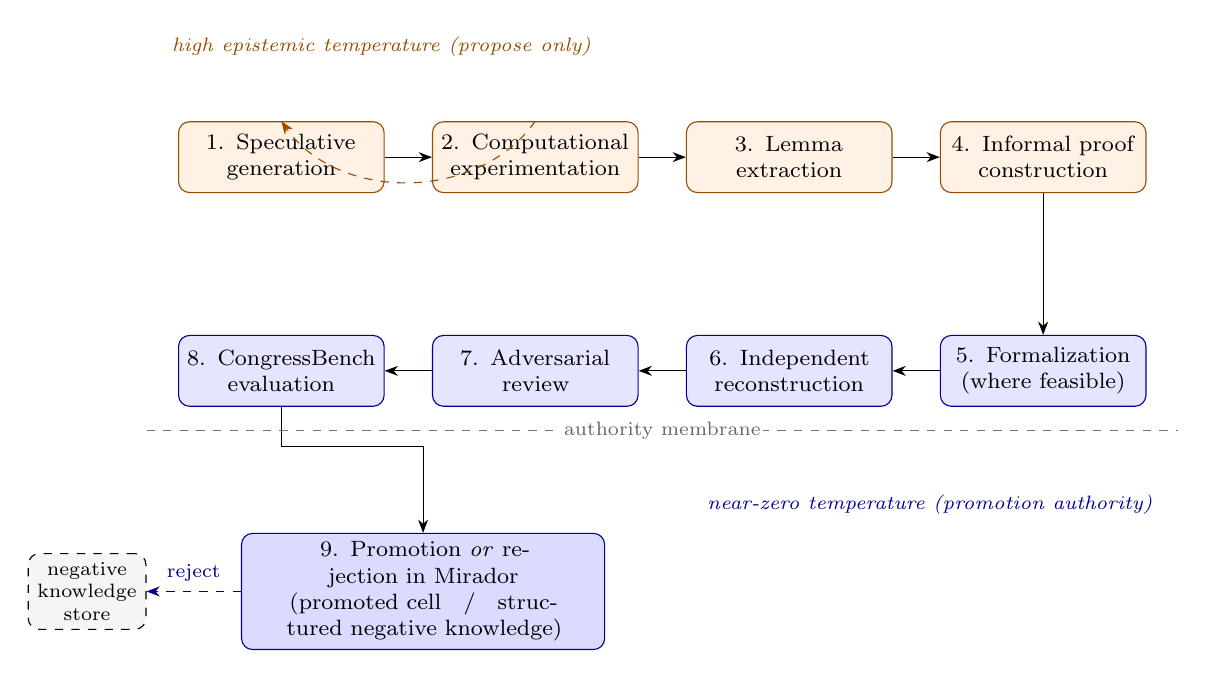
\begin{tikzpicture}[
    font=\footnotesize,
    stage/.style={draw, rounded corners, align=center, minimum height=9mm,
                  text width=24mm, inner sep=3pt},
    sgen/.style={stage, fill=orange!10, draw=orange!60!black},
    strust/.style={stage, fill=blue!10, draw=blue!60!black},
    >=Stealth, node distance=6mm,
    ]
\node[sgen] (s1) {1. Speculative\\generation};
\node[sgen, right=of s1] (s2) {2. Computational\\experimentation};
\node[sgen, right=of s2] (s3) {3. Lemma\\extraction};
\node[sgen, right=of s3] (s4) {4. Informal proof\\construction};

\node[strust, below=18mm of s4] (s5) {5. Formalization\\(where feasible)};
\node[strust, left=of s5] (s6) {6. Independent\\reconstruction};
\node[strust, left=of s6] (s7) {7. Adversarial\\review};
\node[strust, left=of s7] (s8) {8. CongressBench\\evaluation};

\node[strust, below=16mm of s8, xshift=18mm, text width=44mm, fill=blue!14] (s9)
     {9. Promotion \emph{or} rejection in Mirador\\ \footnotesize(promoted cell \; / \; structured negative knowledge)};

% negative-knowledge sink (rejection is retained, not deleted)
\node[draw, dashed, rounded corners, fill=gray!8, align=center, font=\scriptsize,
      left=12mm of s9, anchor=east] (nk) {negative\\knowledge\\store};

\draw[->] (s1) -- (s2);
\draw[->] (s2) -- (s3);
\draw[->] (s3) -- (s4);
\draw[->] (s4) -- (s5);
\draw[->] (s5) -- (s6);
\draw[->] (s6) -- (s7);
\draw[->] (s7) -- (s8);
\draw[->] (s8.south) -- ++(0,-5mm) -| (s9.north);

% early refutation feedback (unlabelled; explained in the caption)
\draw[->, orange!60!black, dashed] (s2.north) to[bend left=55] (s1.north);
% rejection retained as negative knowledge
\draw[->, blue!55!black, dashed] (s9.west) -- (nk.east)
      node[midway, above, font=\scriptsize]{reject};

% authority membrane (between the two rows), label masked over the line
\draw[dashed, black!55] ($(s8.south west)+(-4mm,-3mm)$) -- ($(s5.south east)+(4mm,-3mm)$);
\node[font=\scriptsize, black!60, fill=white, inner sep=1pt]
      at ($(s8.south east)!0.5!(s5.south west)+(0,-3mm)$) {authority membrane};

% temperature labels, in the empty corners
\node[font=\scriptsize\itshape, orange!60!black, anchor=south west] at ($(s1.north west)+(-2mm,7mm)$)
     {high epistemic temperature (propose only)};
\node[font=\scriptsize\itshape, blue!60!black, anchor=north east] at ($(s5.south east)+(2mm,-10mm)$)
     {near-zero temperature (promotion authority)};
\end{tikzpicture}
}
\caption{The discovery-to-promotion lifecycle. Stages 1--4 are high-temperature and propose-only;
the authority membrane precedes formalization; stages 5--8 are near-zero-temperature and
independent. A counterexample at stage 2 refutes early and cheaply; a rejection at stage 9 is stored
as structured negative knowledge and fed back to the Frontier Atlas.}
\label{fig:lifecycle}
\end{figure}

% =====================================================================
\section{Typed Epistemic Representation}
\label{sec:repr}

\PF{} does not invent a knowledge model; it extends Mirador's. The unit remains the typed, versioned
Mathematical Cell, with object type orthogonal to epistemic state and identity given by the canonical
hash of statement-plus-context. \PF{} adds node types and relation types adequate to techniques,
bridges, concepts, failures, and candidate domains (Table~\ref{tab:nodes}). The full JSON schema is
in Appendix~\ref{app:schema}.

\begin{table}[t]
\centering
\small
\caption{\PF{} extension of the Mirador type system. Node types (left) and relation types (right)
adequate to theory formation. All are represented as typed, versioned cells / edges; object type
remains orthogonal to epistemic state.}
\label{tab:nodes}
\begin{tabular}{p{0.46\textwidth} p{0.46\textwidth}}
\toprule
\textbf{Node types} & \textbf{Relation types} \\
\midrule
\ntype{MathematicalObject}, \ntype{Definition}, \ntype{Invariant}, \ntype{Technique},
\ntype{ProofSchema}, \ntype{Analogy}, \ntype{Translation}, \ntype{Obstruction},
\ntype{Counterexample}, \ntype{FailedApproach}, \ntype{ResearchBottleneck}, \ntype{ConceptualGap},
\ntype{UnexplainedPattern}, \ntype{CandidateDomain}, \ntype{ValidationArtifact}
&
\rel{analogous\_to}, \rel{transports\_to}, \rel{preserves}, \rel{breaks\_under},
\rel{generalizes}, \rel{specializes}, \rel{dualizes}, \rel{compresses}, \rel{predicts},
\rel{solves\_bottleneck}, \rel{is\_obstructed\_by}, \rel{fails\_because}, \rel{depends\_on},
\rel{independently\_reproduced\_by} \\
\bottomrule
\end{tabular}
\end{table}

\paragraph{Object specification.} Every \PF{} object carries, in addition to the Mirador core, the
following fields (semi-formally; see Appendix~\ref{app:schema}):
\begin{itemize}[leftmargin=1.4em,itemsep=1pt]
  \item \textbf{identity} --- canonical hash of the identity-bearing statement-plus-context (a
  renamed object collides with its source);
  \item \textbf{version} --- content hash plus environment (the versioned definitions it is stated
  against);
  \item \textbf{provenance} --- generating operator, parent cells, Evidence-Bundle hash, model /
  prompt / seed, primary sources with access dates;
  \item \textbf{assumptions} --- the identity-bearing context $\Gamma$;
  \item \textbf{evidence} / \textbf{counterevidence} --- supporting and adversarial examples, tested
  ranges, known counterexamples;
  \item \textbf{epistemic\_status} --- one of the Mirador states (\state{DRAFT} $\to$ \state{OPEN}
  $\to$ \state{EVIDENCE} $\to \dots \to$ \state{PROMOTED}, with \state{REFUTED}, \state{NO\_GO},
  \state{SUSPECT});
  \item \textbf{novelty\_status} --- the novelty vector of \S\ref{sec:novelty}, never a single
  scalar authority;
  \item \textbf{formalization\_status} --- \{unformalized, informal-proof, formalized, certified\},
  with an informal--formal \emph{correspondence} record that is never inferred from successful
  compilation;
  \item \textbf{reproducibility\_status} --- whether an independent agent reconstructed the object;
  \item \textbf{promotion\_history} --- the append-only log of state transitions and the review
  independence at each promotion.
\end{itemize}

\paragraph{Negative knowledge as typed objects.} \ntype{FailedApproach}, \ntype{Obstruction}, and
\ntype{Counterexample} are first-class node types with a \rel{fails\_because} relation to the target
they do not solve and a \rel{breaks\_under} relation to the conditions that defeat them. A
bridge-failure certificate is a \ntype{ValidationArtifact} attached to an \ntype{Analogy} or
\ntype{Translation}. This is what makes Principle~\ref{prin:failure} mechanical rather than
aspirational, and is the substrate for RQ6.

Figure~\ref{fig:casegraph} shows a small typed graph fragment for the illustrative campaign of
\S\ref{sec:case}, exhibiting the node and relation types in use.

\begin{figure}[t]
\centering
\resizebox{0.92\textwidth}{!}{% Typed epistemic graph fragment for the illustrative campaign (affine plank).
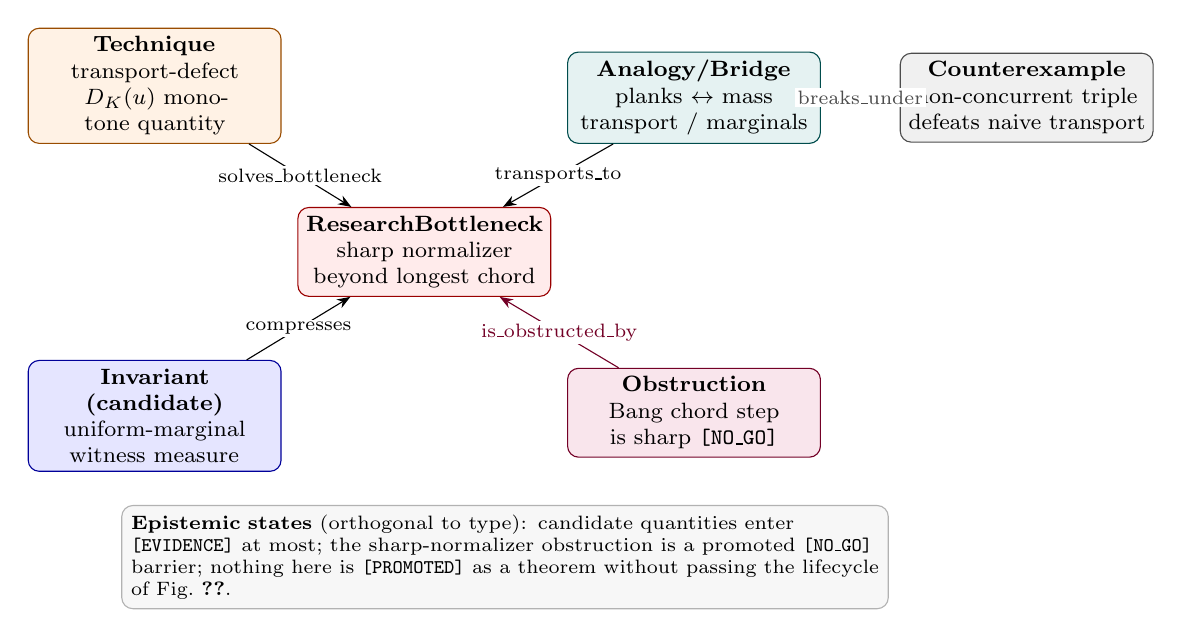
\begin{tikzpicture}[
    font=\footnotesize,
    n/.style={draw, rounded corners, align=center, inner sep=3pt,
              minimum height=7mm, text width=30mm},
    bott/.style={n, fill=red!8, draw=red!60!black},
    tech/.style={n, fill=orange!10, draw=orange!60!black},
    bridge/.style={n, fill=teal!10, draw=teal!60!black},
    concept/.style={n, fill=blue!10, draw=blue!60!black},
    cex/.style={n, fill=gray!12, draw=gray!60!black},
    obs/.style={n, fill=purple!10, draw=purple!60!black},
    >=Stealth,
    every edge quotes/.style={font=\scriptsize, fill=white, inner sep=1pt},
    ]
\node[bott] (b) {\textbf{ResearchBottleneck}\\\footnotesize sharp normalizer beyond longest chord};
\node[tech, above left=8mm and 2mm of b] (t) {\textbf{Technique}\\\footnotesize transport-defect $D_K(u)$ monotone quantity};
\node[bridge, above right=8mm and 2mm of b] (br) {\textbf{Analogy/Bridge}\\\footnotesize planks $\leftrightarrow$ mass transport / marginals};
\node[concept, below left=8mm and 2mm of b] (c) {\textbf{Invariant (candidate)}\\\footnotesize uniform-marginal witness measure};
\node[obs, below right=9mm and 2mm of b] (o) {\textbf{Obstruction}\\\footnotesize Bang chord step is sharp \texttt{[NO\_GO]}};
\node[cex, right=10mm of br] (cex) {\textbf{Counterexample}\\\footnotesize non-concurrent triple defeats naive transport};

\draw[->] (t) edge["solves\_bottleneck"] (b);
\draw[->] (br) edge["transports\_to"] (b);
\draw[->] (c) edge["compresses"] (b);
\draw[->, purple!60!black] (o) edge["is\_obstructed\_by" {swap}] (b);
\draw[->, gray!60!black] (cex) edge["breaks\_under" {swap}] (br);

\node[font=\scriptsize, align=left, draw=black!30, rounded corners, fill=black!3,
      below=6mm of o, xshift=-24mm, text width=95mm]
     {\textbf{Epistemic states} (orthogonal to type): candidate quantities enter \texttt{[EVIDENCE]} at most;
      the sharp-normalizer obstruction is a promoted \texttt{[NO\_GO]} barrier; nothing here is \texttt{[PROMOTED]}
      as a theorem without passing the lifecycle of Fig.~\ref{fig:lifecycle}.};
\end{tikzpicture}
}
\caption{A typed epistemic-graph fragment for the illustrative campaign (\S\ref{sec:case}). Node
types and relations are drawn from Table~\ref{tab:nodes}; epistemic states are orthogonal to type.
Candidate quantities enter \state{EVIDENCE} at most; the sharp-normalizer result is a promoted
\state{NO\_GO} barrier; nothing is \state{PROMOTED} as a theorem without passing the lifecycle of
Fig.~\ref{fig:lifecycle}.}
\label{fig:casegraph}
\end{figure}

% =====================================================================
\section{Mathematical Novelty and Promotion Criteria}
\label{sec:novelty}

By Principle~\ref{prin:novelty}, \PF{} does not reduce novelty to textual distance, embedding
distance, or absence from a retrieval corpus. It reports a \emph{vector} of dimensions and gates
promotion on a conjunction of criteria, not a threshold on a scalar.

\subsection{Novelty dimensions}

\begin{description}[leftmargin=1.4em,itemsep=1pt]
  \item[Structural novelty] change in the typed structure of objects / relations, not their names.
  \item[Operational novelty] a genuinely new operation (a new technique operator, a new transport),
  as opposed to a re-parameterisation of an existing one.
  \item[Explanatory compression] reduction in the number of independent conditions or lemmas needed
  to state or prove a family of results.
  \item[Theorem productivity] the number and depth of new theorems the object yields.
  \item[Transfer breadth] the number of distinct problem families or domains the object reaches.
  \item[Counterfactual necessity] whether an ablation shows the new component is required
  (Principle~\ref{prin:necessity}).
  \item[Robustness] stability of the object's value under perturbation of examples and hypotheses.
  \item[Independent rediscovery] whether an agent with no shared context reconstructs the object.
  \item[Formal-verification coverage] the fraction of the object's claims that are formalized or
  certified.
  \item[Proof-complexity reduction] shortening of proofs that use the object.
  \item[Hypothesis-complexity reduction] weakening of hypotheses that the object enables.
\end{description}

\subsection{Scoring, and why no scalar suffices}

We propose a scoring model that reports the above as a labelled vector and, \emph{only for scheduler
allocation}, a preregistered scalar aggregate. The scalar never decides promotion. The reason is
structural: the dimensions are not commensurable and can move in opposite directions---a concept can
have high explanatory compression yet zero independent rediscovery, or high theorem productivity on
the training examples yet no held-out transfer. Collapsing them hides exactly the failure modes the
system exists to catch. Promotion is therefore gated on a \emph{conjunction} of criteria appropriate
to the object's level (\S\ref{sec:governance}, Appendix~\ref{app:gates}), not on a scalar threshold.

\subsection{Anti-gaming detection}

\PF{} includes explicit mechanisms to detect the ways an unsupervised generator can fake novelty
(Table~\ref{tab:antigaming}). Several are inherited mechanically from Mirador (content-hash identity,
acyclicity-of-justification audit); the rest are dedicated checks.

\begin{table}[t]
\centering
\small
\caption{Failure modes of automated novelty and the mechanism that detects each.}
\label{tab:antigaming}
\begin{tabular}{p{0.42\textwidth} p{0.52\textwidth}}
\toprule
\textbf{Failure mode} & \textbf{Detection mechanism} \\
\midrule
Cosmetic renaming & content-hash identity collision (Mirador); flagged non-novel \\
Disguised restatement & semantic-equivalence check to exposed cells; requires certified link, never
inferred \\
Trivial generalization & zero theorem yield \emph{and} failed necessity ablation \\
Memorized rediscovery & memorization probe; author-perturbed variants with unpublished surface form \\
Benchmark contamination & held-out splits; sealed test run once; contamination controls
(\S\ref{sec:bench}) \\
Circular definitions & acyclicity-of-justification audit (Mirador) \\
Analogy without transport & BridgeForge gate: no transported theorem $\Rightarrow$ reject
(Principle~\ref{prin:transport}) \\
Concept fitted to selected examples & held-out predictive test; perturbation robustness \\
\bottomrule
\end{tabular}
\end{table}

\subsection{Promotion criteria by level}

\begin{criterion}[Technique, $L1$]
Necessity ablation passes; the technique closes a stated obligation; independent reconstruction
succeeds; adversarial review finds no unresolved material objection.
\end{criterion}
\begin{criterion}[Bridge, $L2$]
At least one nontrivial theorem is transported with a discharged proof obligation; a testable
prediction is confirmed by Experimentarium; a bridge-failure certificate is present; review passes.
\end{criterion}
\begin{criterion}[Concept, $L3$]
Explanatory compression is demonstrated; held-out predictive utility exceeds a preregistered
baseline; nontriviality (not a renamed known object) is established; review passes.
\end{criterion}
\begin{criterion}[Candidate domain, $L4$]
The longitudinal productivity criteria of \S\ref{sec:domainfoundry} are met over a fixed horizon,
including use by an independent agent and transfer to an established domain; adjudicated externally,
never self-declared.
\end{criterion}

% =====================================================================
\section{ParadigmForgeBench}
\label{sec:bench}

\pfbench{} is an evaluation framework---not a fixed dataset with a leaderboard---for the four levels
of novelty. It has four tracks (Fig.~\ref{fig:tracks}). Each track specifies a task construction, a
pass criterion tied to a promotion criterion, and contamination controls. \textbf{No track has been
run}; task banks and sealed sets are to be built and frozen under the roadmap.

\begin{figure}[t]
\centering
\resizebox{\textwidth}{!}{% ParadigmForgeBench: four evaluation tracks with what each demands.
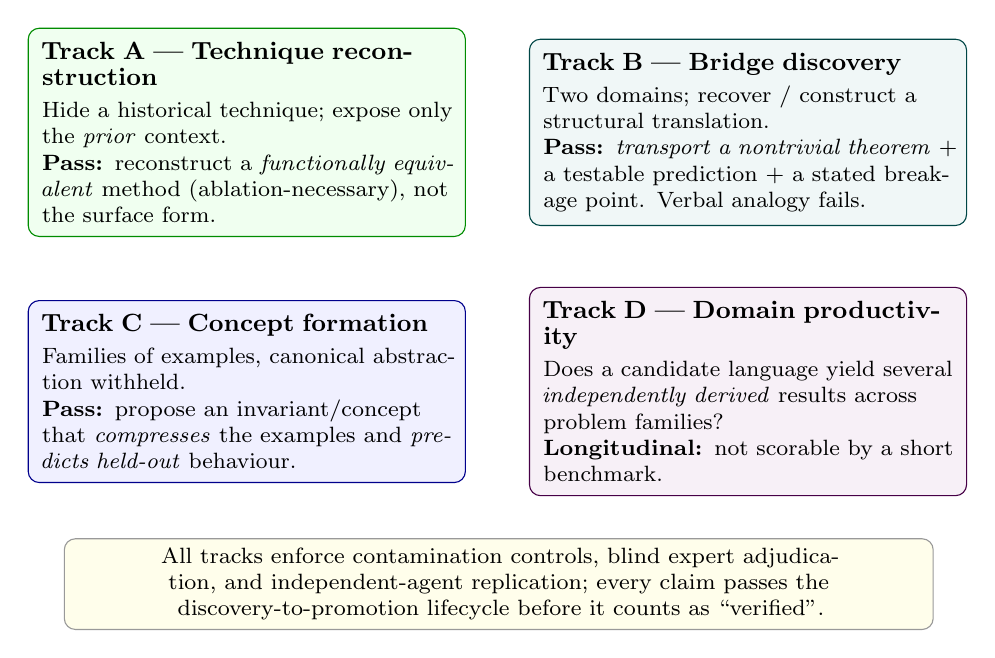
\begin{tikzpicture}[
    font=\footnotesize,
    trk/.style={draw, rounded corners, align=left, inner sep=5pt,
                text width=52mm, minimum height=20mm, fill=gray!5},
    hd/.style={font=\small\bfseries},
    >=Stealth,
    ]
\node[trk, draw=green!55!black, fill=green!6] (a)
  {{\bfseries\small Track A --- Technique reconstruction}\\[2pt]
   Hide a historical technique; expose only the \emph{prior} context.\\
   \textbf{Pass:} reconstruct a \emph{functionally equivalent} method (ablation-necessary), not the surface form.};
\node[trk, draw=teal!55!black, fill=teal!6, right=8mm of a] (b)
  {{\bfseries\small Track B --- Bridge discovery}\\[2pt]
   Two domains; recover / construct a structural translation.\\
   \textbf{Pass:} \emph{transport a nontrivial theorem} + a testable prediction + a stated breakage point. Verbal analogy fails.};
\node[trk, draw=blue!55!black, fill=blue!6, below=8mm of a] (c)
  {{\bfseries\small Track C --- Concept formation}\\[2pt]
   Families of examples, canonical abstraction withheld.\\
   \textbf{Pass:} propose an invariant/concept that \emph{compresses} the examples and \emph{predicts held-out} behaviour.};
\node[trk, draw=violet!55!black, fill=violet!6, right=8mm of c] (d)
  {{\bfseries\small Track D --- Domain productivity}\\[2pt]
   Does a candidate language yield several \emph{independently derived} results across problem families?\\
   \textbf{Longitudinal:} not scorable by a short benchmark.};

\node[draw=black!40, rounded corners, fill=yellow!8, below=7mm of c, xshift=32mm,
      text width=108mm, align=center, font=\footnotesize] (note)
  {All tracks enforce contamination controls, blind expert adjudication, and independent-agent replication; every claim passes the discovery-to-promotion lifecycle before it counts as ``verified''.};
\end{tikzpicture}
}
\caption{The four \pfbench{} tracks. A--C are the primary quantitative tracks; D is longitudinal and
reported qualitatively against preregistered milestones. Every track enforces contamination controls,
blind expert adjudication, and independent-agent replication.}
\label{fig:tracks}
\end{figure}

\subsection{Track A: Technique reconstruction}
Hide a historically important technique while exposing \emph{only} the mathematical context that
preceded it, and evaluate whether the system reconstructs a functionally equivalent method.
Candidate retrospective cases---used only where the pre-discovery context can be cleanly
reconstructed and the contamination risk is documented---include diagonalization, generating
functions, the probabilistic method, monotonicity-quantity mechanisms in geometric flows, the
polynomial method, forcing, and Fourier-analytic techniques in additive combinatorics
\citep{cohen1963,greentao2008,guthkatz2015,hamilton1982,perelman2002}. The pass criterion is
\emph{functional}: an ablation shows the reconstructed technique's novel component is necessary to
close the target obligation (Principle~\ref{prin:necessity}); textual match to the historical
statement is neither necessary nor sufficient. The first-order threat is contamination: every base
technique is public and memorised by modern models, so the track requires a memorization probe run
before scoring and author-perturbed variants whose surface form was never published. This track
operationalises RQ1.

\subsection{Track B: Bridge discovery}
Provide two domains with a known (withheld) structural correspondence and a set of decoy pairs, and
test whether the system recovers or constructs a meaningful translation. Evaluation requires
\emph{theorem transport}, not verbal analogy: a pass requires a typed alignment that transports at
least one nontrivial theorem with a checkable obligation, a confirmed testable prediction, and a
bridge-failure certificate. This track operationalises RQ2.

\subsection{Track C: Concept formation}
Provide families of examples with the canonical abstraction withheld and a held-out split, and test
whether the system proposes an invariant or concept that compresses the visible examples and
\emph{predicts held-out behaviour} above a preregistered baseline, while surviving the overfitting
probes of \S\ref{sec:novelty}. This track operationalises RQ3.

\subsection{Track D: Domain productivity}
Evaluate whether a candidate conceptual language supports several \emph{independently derived}
results across multiple problem families over a fixed horizon. Full ``new branch creation'' cannot
be evaluated by a short benchmark: it is defined by sustained autonomous productivity and must be
assessed \emph{longitudinally}, with preregistered milestones (number of independent theorems,
distinct problem families, internal questions, transfer, and use by a non-proposer agent), never as
a single success rate. This track operationalises RQ5.

% =====================================================================
\section{Experimental Methodology}
\label{sec:method}

We describe a credible empirical program. \textbf{It is proposed, not executed}; the full phase
schedule, blocking decisions, and preregistration ritual are in the accompanying roadmap. The
purpose here is to make the architecture falsifiable.

\paragraph{Design.} Retrospective rediscovery experiments (Track A); held-out mathematical domains
(Tracks B, C); contamination controls (memorization probes, perturbed variants, sealed test run
once); blind expert evaluation; independent-agent replication; adversarial counterexample search;
formal verification where possible; and comparison against strong baselines: a direct language-model
prover/reasoner, a retrieval-only system, unguided multi-agent debate, and TheoryForge without the
\PF{} layer. Compute and inference budgets are reported for every arm.

\paragraph{Ablations.} The program removes, one at a time: the Frontier Atlas (undirected
exploration); negative knowledge; BridgeForge; Experimentarium (no computational falsification
pressure); independent review (self-review only); Mirador's typed representation (prose cells);
formal verification; and the domain-transfer requirement. The central governance test (RQ4) is
whether removing independent review \emph{raises} the \ftpr{} and the cosmetic-novelty escape rate;
the negative-knowledge test (RQ6) is whether removing the failure store increases repeated failure
and time-to-first-useful-candidate.

\paragraph{Statistics.} Comparisons are paired on shared items (clustered by base problem/domain),
with the design effect reported; effect sizes with intervals, not only $p$-values; multiplicity
controlled; the sealed test executed once with no optional stopping. Every table regenerates
deterministically from raw artifacts.

\paragraph{Placeholders, not results.} Table~\ref{tab:pending} shows the frozen shape of the primary
results reporting. \textbf{Its cells are intentionally empty}; they are filled only after
preregistration freeze and the runs specified in the roadmap. Nothing in this paper is a finding.

\begin{table}[t]
\centering
\small
\caption{\textbf{[PENDING --- no experiment run]} Frozen shape of the primary \pfbench{} results.
Cells are filled only after preregistration freeze; this is a reporting template, not data.}
\label{tab:pending}
\resizebox{\textwidth}{!}{%
\begin{tabular}{l l c c c c}
\toprule
Track & Arm & Pass rate & Necessity-ablation & Transfer & Compute (rel.) \\
\midrule
A (technique) & B-LLM / B-RET / B-DEBATE / B-TF / PF & \emph{[pending]} & \emph{[pending]} & --- & \emph{[pending]} \\
B (bridge) & B-LLM / B-RET / B-DEBATE / B-TF / PF & \emph{[pending]} & --- & \emph{[pending]} & \emph{[pending]} \\
C (concept) & B-LLM / B-RET / B-DEBATE / B-TF / PF & \emph{[pending]} & --- & \emph{[pending]} & \emph{[pending]} \\
D (domain) & PF (longitudinal) & \multicolumn{4}{c}{\emph{[longitudinal --- milestone trajectory, not a scalar]}} \\
\bottomrule
\end{tabular}}
\end{table}

% =====================================================================
\section{Illustrative Research Campaign}
\label{sec:case}

We give a technically serious illustration of the workflow on an open but tractable problem already
documented in the Bourbaki corpus: \emph{Bang's affine plank problem}
\citep{bang1951,ball1991,gardner1988,lucius2026bang}. The purpose is to demonstrate the components in
motion, \emph{not} to solve the problem. It is academically legitimate---and here more
informative---for the illustration to end in a structured, well-explained non-result.

\paragraph{The problem.} A \emph{plank} of width $w$ is the region between two parallel hyperplanes
at distance $w$. For a convex body $K$ and a plank $P$ with normal $u$, the relative width is
$\mathrm{rw}_K(P) = \mathrm{width}(P)/\mathrm{width}_K(u)$. Bang's affine plank conjecture (1951)
asserts that if $K$ is covered by planks $P_1,\dots,P_n$ then $\sum_i \mathrm{rw}_K(P_i) \ge 1$.
Ball proved the centrally symmetric case \citep{ball1991}; the general (affine) case is open, already
in the plane and already for three planks, and Gardner posed the associated relative-width
witness-measure existence question \citep{gardner1988}.

\paragraph{1. Frontier Atlas.} Ingesting the plank literature and the documented campaign
\citep{lucius2026bang}, the Atlas assembles known results (Ball's symmetric theorem; the
transport-defect framework $D_K(u)$; a median theorem with rigidity on the triangle; a
three-direction characterization settling Gardner's question for three directions), techniques and
their regimes, and barriers.

\paragraph{2. Bottleneck.} The Atlas localises a precise \ntype{ResearchBottleneck}: existing
arguments control the covering constant only up to the \emph{one-plank-per-direction} restriction
($C^{111}$), and the step that would extend a bound to the unrestricted constant $C$ passes through a
normalizer argument that is \emph{sharp}---Bang's chord-lemma step cannot reach any normalizer beyond
the longest chord. The bottleneck cell names exactly this obligation: transport a bound from
$C^{111}$ to $C$ without the chord-lemma normalizer. (This is also the site of the campaign's
documented flagship defect: a value proved for $C^{111}$ but stated for $C$, where $C \le C^{111}$
makes the two non-interchangeable \citep{lucius2026mirador}.)

\paragraph{3. Candidate technique (TechniqueForge).} A candidate technique proposes to
\emph{quantitatively strengthen} the transport-defect argument by coupling energy-type estimates to a
concentration-of-measure control on the marginal defect, aiming for an almost-monotone quantity that
survives the passage from $C^{111}$ to $C$. The candidate is emitted at \state{EVIDENCE} with a
necessity-ablation obligation: remove the concentration control and check whether the transport step
still closes.

\paragraph{4. Candidate bridge (BridgeForge).} A candidate \ntype{Analogy}/\ntype{Translation}
aligns plank coverings with a mass-transport / marginal-coupling formulation: planks and directions
map to marginals, relative width to a transport cost, and the covering inequality to a
marginal-defect bound. The bridge is required to \emph{transport} a nontrivial statement (e.g.\ the
symmetric case's marginal identity) and to emit a failure certificate. Experimentarium immediately
supplies a candidate \ntype{Counterexample}: a non-concurrent tilted triple defeats the naive
transport, so the bridge is annotated \rel{breaks\_under} ``non-concurrent triples'' rather than
promoted.

\paragraph{5. Candidate invariant (ConceptForge).} A candidate \ntype{Invariant}---a uniform-marginal
witness measure whose existence is equivalent to a concurrence condition on mid-level lines---is
proposed as the object that \rel{compresses} the three-direction phenomena. It is computed on known
cases and scored on explanatory compression and held-out prediction; on the triangle it recovers the
documented three-direction characterization but does \emph{not}, in this illustration, extend to
general triples.

\paragraph{6. Computational tests (Experimentarium).} Finite enumeration and exact-rational
certificate search stress the candidates: the one-plank-per-direction constant at a specific tilted
triple is confirmed by an independent checker over a large exact certificate
\citep{lucius2026bang}, while the unrestricted constant remains open; the candidate almost-monotone
quantity fails to remain monotone on a perturbed family, producing falsification pressure rather than
support.

\paragraph{7. Lemma extraction.} The \ntype{MinimalMissingLemma} is extracted: a ``thin-plank''
lemma that would lift the finite branch-and-bound to the full cyclic family. It is emitted
\state{OPEN} with a \rel{solves\_bottleneck} edge---the precise statement whose absence blocks the
campaign.

\paragraph{8. Adversarial objections.} A fresh-context review (CongressBench-conforming) raises:
(i) the transported statement in step 4 holds only under concurrence (scope objection); (ii) the
almost-monotone quantity is not monotone off the perturbed family (necessity-ablation failure);
(iii) the $C^{111}$-vs-$C$ scope must not be elided (the documented flagship defect). Each objection
is a structured veto with a discharge condition.

\paragraph{9. Outcome.} The honest outcome of this illustration is a \emph{structured non-result}:
the sharp-normalizer obstruction is promoted as a \state{NO\_GO} \emph{barrier} (a first-class asset
that prunes an entire method family); the candidate technique and bridge are \state{REFUTED} on the
perturbed family and stored as \ntype{FailedApproach} with \rel{fails\_because} explanations; the
uniform-marginal invariant is retained at \state{EVIDENCE} for three directions with an explicit
non-extension note; and the thin-plank lemma is recorded as the ranked next target. No theorem is
promoted, no problem is claimed solved, and the negative knowledge produced is precisely the material
that sharpens the Frontier Atlas for the next cycle (RQ6). Figure~\ref{fig:casegraph} shows the
resulting typed graph fragment.

% =====================================================================
\section{Governance, Failure and Negative Knowledge}
\label{sec:governance}

Governance is what separates \PF{} from an ideation loop. Three mechanisms carry it.

\paragraph{Separation of powers.} By Principle~\ref{prin:temp}, generation and promotion are distinct
authorities and never vested in the same agent. A discovery agent may propose an object at
\state{DRAFT}/\state{EVIDENCE}; only the independent review body may promote, and only through the
Mirador transition table, which mechanically forbids self-promotion and requires a fresh-context
reviewer at independence level $\ge 3$ with no unresolved veto \citep{lucius2026mirador}. In the
implementation this is a database-permission fact, not a policy request: the generating role holds no
write access to the promoted corpus \citep{lucius2026bourbaki}.

\paragraph{Adversarial review.} Promotion runs through a CongressBench-conforming panel
\citep{lucius2026congressbench} whose lenses are tuned to \PF{}'s failure modes: a necessity-ablation
auditor (was the new component required?); a transport auditor (does the bridge carry a theorem?); a
scope/assumption auditor (the $C^{111}$-vs-$C$ lens); a novelty-and-priority auditor (is this a
renamed known object?); and an independent-reconstruction auditor. Whether fresh-context review
lowers the \ftpr{} relative to shared-context review is the empirical wager the companion benchmark
is built to settle; \PF{} inherits it as a hypothesis (RQ4), not a fact.

\paragraph{Negative knowledge as a first-class output.} By Principle~\ref{prin:failure}, rejection is
recorded, not discarded. A refuted technique becomes a \ntype{FailedApproach} with a
\rel{fails\_because} edge; a defeated bridge yields a bridge-failure \ntype{ValidationArtifact}; a
proved impossibility becomes a \ntype{Obstruction} in state \state{NO\_GO}, valued at parity with a
positive result because it prunes infinite search. The Frontier Atlas consumes these directly: a
family of approaches that fail for a common reason collapses to one high-value cell, so the system
does not re-attempt known-dead routes. This is the mechanism behind RQ6, and it is the
counterpart, at the level of theory formation, of the invalidation propagation that Mirador provides
at the level of claims.

% =====================================================================
\section{Limitations and Threats to Validity}
\label{sec:limits}

We state the limitations bluntly, because the paper's credibility depends on not overclaiming.

\paragraph{Maturity.} \PF{} is \emph{specified, not built}. The substrates it depends on (Mirador,
ProofContext) are implemented prototypes; the six \PF{} components, the type-system extension, and
\pfbench{} are designs. Two dependencies are known blockers: ProofContext currently exposes neither
cross-domain analogy retrieval nor a collision-search client, which are prerequisites for BridgeForge
and for the first novelty-screening stage \citep{lucius2026theoryforge}. No \PF{} experiment has been
run.

\paragraph{No results.} This paper contains no accuracy, success rate, expert assessment, quotation,
table of measurements, or mathematical discovery. Every results table is a labelled placeholder.
Claims are architectural and methodological only.

\paragraph{Contamination.} The retrospective tracks rely on techniques and problems that are public
and memorised by modern models. Contamination is mitigated (memorization probes, perturbed variants,
functional rather than textual scoring, sealed tests) but cannot be eliminated; Track A results, once
produced, must be read with that caveat, and rediscovery must never be reported as novelty.

\paragraph{Evaluation of the hardest levels.} $L4$ (domain genesis) is not evaluable by any short
benchmark and is deliberately left to longitudinal, external assessment. Even Tracks A--C, being
built by the same program that designs the mechanisms they reward, carry a construct-validity risk
that only a held-out or third-party benchmark can resolve.

\paragraph{The generator is a bound.} \PF{} does not manufacture insight. A campaign is bounded by
the best technique, bridge, or concept its generators can propose, and by representation bottlenecks,
formalization cost, retrieval error, and model homogenisation. Governance can prevent false
promotion; it cannot create tractability.

\paragraph{Anthropomorphism.} We avoid claims of ``mathematical creativity'' or ``understanding''.
\PF{} proposes candidate objects and governs their validation; whether the resulting process
resembles human discovery is out of scope.

% =====================================================================
\section{Relationship with the Clay Millennium Problems}
\label{sec:millennium}

We discuss the Millennium Prize Problems only as a long-term motivating horizon, and we make no claim
that \PF{} can solve one. The reason to mention them is that they are precisely the class of problems
for which proving-in-a-fixed-language is plausibly insufficient. Several may require
\emph{new techniques}, \emph{unexpected bridges}, \emph{new conceptual languages}, or frameworks not
yet available---the very objects \PF{} is designed to propose and govern. Historically, decisive
progress on hard problems has come through exactly such representational change: forcing for the
continuum hypothesis \citep{cohen1963}, Ricci-flow monotonicity for the geometrisation and Poincar\'e
programs \citep{hamilton1982,perelman2002}, the polynomial method for incidence problems
\citep{guthkatz2015}, and Fourier-analytic transference in additive combinatorics
\citep{greentao2008}.

Two distinctions matter. First, olympiad problem solving is not research-level theory formation: the
former discharges statements in a settled language under time pressure
\citep{trinh2024alphageom,chervonyi2025alphageom2}; the latter changes the language---closer in
spirit to research-level benchmarks of unpublished problems \citep{abouzaid2026firstproof}---and its
success predicate is external and slow. Second, a Millennium ``solution'' cannot be defined by an internal
agent verdict: it is closed only by the external mathematical process (journal acceptance, community
validation), which no system can short-circuit \citep{lucius2026bourbaki}. \PF{} is therefore
positioned not as a solver but as a test of whether AI can participate in \emph{constructing the
conceptual machinery} that frontier problems may require---and, just as importantly, of whether that
participation can be governed so that its speculative output does not contaminate trusted knowledge.

% =====================================================================
\section{Research Roadmap}
\label{sec:roadmap}

The execution plan is preregistered in the accompanying roadmap document; we summarise its spine. The
program proceeds in phases: extend the Mirador schema and validators (P0); build the Frontier Atlas
over a frozen corpus (P1); implement Experimentarium with exact-arithmetic re-checking (P2);
implement the TechniqueForge / BridgeForge / ConceptForge operators and the necessity-ablation
harness (P3); \emph{freeze} the preregistration---protocols, corpora manifests, ablation matrix,
novelty-rubric weights, split hashes---as a hash-pinned event (P4); run Tracks A--C and the
governance ablations (P5--P7); pilot the longitudinal Track D under external expert governance (P8);
and execute the sealed test once, reporting every number regenerated from raw artifacts, including
null and negative results (P9). Blocking decisions---compute budget, model families for the
independence requirement, retrospective-corpus selection and licensing, the external expert panel,
the held-out concept/bridge targets, and the ProofContext analogy/collision extensions---are
enumerated there and must be signed off before P4.

% =====================================================================
\section{Conclusion}
\label{sec:conclusion}

\PF{} extends the Bourbaki Engine from the governance of claim promotion to the governance of theory
formation. Its wager is that progress toward autonomous mathematical discovery requires systems that
can change the representational and conceptual space in which problems are posed---not only prove
statements inside a fixed language---and that such change is safe only under an explicit separation of
temperatures: permissive, diverse, contradictory exploration on one side; conservative, auditable,
independent promotion on the other; every rejection retained as knowledge. We have specified an
architecture for this (Frontier Atlas, TechniqueForge, BridgeForge, ConceptForge, Experimentarium,
DomainFoundry), a typed representation for techniques, bridges, concepts, and failures, a
multidimensional novelty model with explicit anti-gaming controls, and \pfbench{}, a four-track
evaluation framework that measures productivity rather than textual novelty. We have been explicit
that the \PF{} layer is not yet implemented and that no experiment has been run; the paper's
contributions are architectural and methodological, and its results tables are placeholders.

The defensible claim is narrow and, we think, correct: mathematical AI will not reach frontier
discovery merely by proving more statements inside fixed languages. It must also learn to propose,
test, reject, and \emph{govern} changes to the conceptual language of mathematics itself. \PF{} is a
design for doing so without letting speculation masquerade as knowledge.

% =====================================================================
\section*{Reproducibility and Availability}
\addcontentsline{toc}{section}{Reproducibility and Availability}
The LaTeX source, figure sources, a README, and the full experimental roadmap accompany this paper.
No datasets or result artifacts are released, because none exist yet: this is a pre-execution
architecture paper. The companion Bourbaki prototypes are separately available
\citep{lucius2026mirador,lucius2026proofcontext}.

\bibliographystyle{plainnat}
\bibliography{references}

\appendix
% =====================================================================
\section{Object Schemas}
\label{app:schema}

A semi-formal specification of the \PF{} extension cell (JSON-like; the executable schema targets
Mirador's \texttt{mirador-cell/1.0} and adds the fields below). Object type is orthogonal to
epistemic state; identity is the canonical hash of the identity-bearing statement and context.

{\footnotesize\begin{verbatim}
ParadigmForgeCell {
  id                    : content-hash(statement + identity-bearing context)   // identity
  version               : hash(content_hash + environment)                     // version axis
  object_type           : one of { MathematicalObject, Definition, Invariant,
                                    Technique, ProofSchema, Analogy, Translation,
                                    Obstruction, Counterexample, FailedApproach,
                                    ResearchBottleneck, ConceptualGap,
                                    UnexplainedPattern, CandidateDomain,
                                    ValidationArtifact }
  epistemic_status      : one of { DRAFT, OPEN, EVIDENCE, CANDIDATE, FORMALIZED,
                                    AUDITED, PROMOTED, REFUTED, NO_GO, SUSPECT,
                                    RETIRED }                    // orthogonal to type
  assumptions           : context Gamma { variables, assumptions, exclusions,
                                          regularity, scope }    // identity-bearing
  statement_ir          : typed intermediate representation      // identity-bearing
  provenance            : { operator, parents[], evidence_bundle_hash,
                            model, prompt, seed, primary_sources[] with access_dates }
  evidence              : { supporting_examples[], tested_range }
  counterevidence       : { adversarial_examples[], known_counterexamples[],
                            unexplained_failures[] }
  novelty_status        : NoveltyVector {                        // never a scalar authority
                            structural, operational, explanatory_compression,
                            theorem_productivity, transfer_breadth,
                            counterfactual_necessity, robustness,
                            independent_rediscovery, formal_coverage,
                            proof_complexity_reduction, hypothesis_complexity_reduction }
  formalization_status  : { unformalized | informal_proof | formalized | certified }
  correspondence_status : { asserted | reviewed | unchecked }   // never inferred from compile
  reproducibility_status: { none | independently_reproduced_by: agent_id }
  edges                 : typed[ analogous_to, transports_to, preserves, breaks_under,
                                 generalizes, specializes, dualizes, compresses,
                                 predicts, solves_bottleneck, is_obstructed_by,
                                 fails_because, depends_on, independently_reproduced_by ]
  promotion_history     : append-only[ {state, actor, review_independence, ts} ]
}
\end{verbatim}}

% =====================================================================
\section{Agent Roles}
\label{app:roles}

\PF{} inherits the Bourbaki role vocabulary and adds theory-formation roles. Generation and
promotion authorities are disjoint (Principle~\ref{prin:temp}).

\begin{itemize}[leftmargin=1.4em,itemsep=1pt]
  \item \textbf{Cartographer} --- builds and maintains the Frontier Atlas; owns \ntype{ResearchBottleneck} cells.
  \item \textbf{Technician} --- runs TechniqueForge operators; emits \ntype{Technique} candidates ($\le$ \state{EVIDENCE}).
  \item \textbf{Bridge-builder} --- runs BridgeForge; emits \ntype{Analogy}/\ntype{Translation} with transport obligations.
  \item \textbf{Conceptor} --- runs ConceptForge; emits \ntype{Definition}/\ntype{Invariant} candidates.
  \item \textbf{Experimenter} --- runs Experimentarium; produces \state{EVIDENCE} and counterexamples, never proof.
  \item \textbf{Formalizer} --- attempts formalization / certificate extraction.
  \item \textbf{Reconstructor} --- an independent agent that re-derives a candidate from scratch (fresh context).
  \item \textbf{Congress (Referees)} --- the only promotion authority; runs the adversarial lenses of \S\ref{sec:governance}.
  \item \textbf{Archivist} --- writes rejections to the negative-knowledge store; owns the event log.
\end{itemize}
No discovery role holds write access to the promoted corpus.

% =====================================================================
\section{Promotion Gates}
\label{app:gates}

Promotion is a conjunction of gates, by level. Each gate is a checkable predicate; failing any gate
returns the object to the speculative zone (or to negative knowledge if refuted).

\begin{table}[h]
\centering
\small
\begin{tabular}{p{0.16\textwidth} p{0.78\textwidth}}
\toprule
Level & Conjunctive promotion gates \\
\midrule
$L1$ Technique & necessity-ablation pass $\wedge$ obligation closed $\wedge$ independent reconstruction $\wedge$ no unresolved veto \\
$L2$ Bridge & $\ge 1$ theorem transported (obligation discharged) $\wedge$ confirmed prediction $\wedge$ failure certificate present $\wedge$ review pass \\
$L3$ Concept & explanatory compression $\wedge$ held-out prediction $>$ baseline $\wedge$ nontriviality (no identity collision) $\wedge$ review pass \\
$L4$ Domain & longitudinal productivity criteria (\S\ref{sec:domainfoundry}) over horizon $\wedge$ independent-agent use $\wedge$ external adjudication \\
\bottomrule
\end{tabular}
\end{table}

% =====================================================================
\section{Evaluation Rubrics}
\label{app:rubrics}

Partial-credit rubrics are reported per dimension, never fused into one number. Sketch:
\begin{itemize}[leftmargin=1.4em,itemsep=1pt]
  \item \textbf{Technique (Track A)} --- \{no candidate; candidate but ablation-unnecessary; necessary
  but obligation not closed; obligation closed; independently reconstructed\}.
  \item \textbf{Bridge (Track B)} --- \{verbal analogy only; typed alignment, no transport; transports
  a trivial statement; transports a nontrivial theorem; transport $+$ confirmed prediction $+$ failure
  certificate\}.
  \item \textbf{Concept (Track C)} --- \{renamed known object; compresses training only; compresses
  $+$ weak held-out; compresses $+$ strong held-out; $+$ transfer to a second family\}.
  \item \textbf{Domain (Track D)} --- milestone trajectory: objects family; internal operations;
  invariants; multi-theorem; multi-family; internal questions; transfer; non-proposer use.
\end{itemize}

% =====================================================================
\section{Example Research Artifacts}
\label{app:artifacts}

Two illustrative negative-knowledge artifacts (schematic; not results).

{\footnotesize\begin{verbatim}
FailedApproach {
  object_type      : FailedApproach
  epistemic_status : REFUTED
  target           : bottleneck: transport bound from C^{111} to C without chord-lemma normalizer
  approach         : almost-monotone quantity via energy + concentration control
  fails_because    : quantity not monotone on the perturbed cyclic family (Experimentarium)
  breaks_under     : { perturbation: off-cyclic tilt }
  reusable         : yes  // prunes the "energy+concentration" family for this bottleneck
}

BridgeFailureCertificate {
  object_type      : ValidationArtifact
  attached_to      : Analogy(planks <-> mass-transport marginals)
  transported      : symmetric-case marginal identity   // holds
  breaks_under      : non-concurrent tilted triples      // transport fails
  prediction_status: refuted by counterexample (Experimentarium)
}
\end{verbatim}}

% =====================================================================
\section{Pseudocode: Discovery and Governance Loops}
\label{app:pseudocode}

The discovery loop (high temperature, propose-only) and the governance loop (near-zero temperature,
promotion authority) are disjoint in authority.

{\footnotesize\begin{verbatim}
# Discovery loop (speculative zone; emits cells <= EVIDENCE only)
def discovery_cycle(target):
    atlas       = FrontierAtlas.build(target, corpus, negative_knowledge)
    bottleneck  = atlas.select_bottleneck()          # ResearchBottleneck
    bundle      = ProofContext.query(bottleneck).bundle
    candidates  = []
    candidates += TechniqueForge.generate(bottleneck, bundle)   # L1
    candidates += BridgeForge.generate(bottleneck, bundle)      # L2
    candidates += ConceptForge.generate(bottleneck, bundle)     # L3
    for c in candidates:
        c = Experimentarium.stress(c)                # evidence + counterexamples, not proof
        if c.refuted:
            NegativeKnowledge.store(c)               # FailedApproach / Obstruction
            continue
        if not necessity_ablation_passes(c):         # Principle: necessity over decoration
            NegativeKnowledge.store(c); continue
        Mirador.write(c, state=EVIDENCE)             # NO promotion authority here
        ReviewQueue.submit(c)
    return

# Governance loop (trust zone; sole promotion authority)
def governance_cycle():
    for c in ReviewQueue:
        assert c.generator != current_reviewer      # separation of powers
        c = Formalizer.try(c)                        # where feasible
        c = Reconstructor.independent(c)             # fresh context
        verdict = Congress.review(c, lenses=[necessity, transport, scope,
                                             novelty_priority, reconstruction])
        if verdict.accept and gates_pass(c, c.level):
            Mirador.promote(c, independence=verdict.level)   # only path to PROMOTED
        else:
            NegativeKnowledge.store(c, reason=verdict.vetoes)  # failure is knowledge
    return
\end{verbatim}}

\end{document}
